\documentclass{beamer}

\usetheme{Madrid}
\usepackage[backend=biber]{biblatex}
\addbibresource{mybib.bib}
\usepackage{graphicx}

\title{Distance Measurement of Objects from 2d Images / Videos}
\author{Ahammed Hani , Dinu D'Silva , Sarath C Ani , Shyamjith M C}


\begin{document}
	
	\maketitle
	
	\section{Introduction}
	\begin{frame}
	\frametitle{Introduction}
	
	\begin{itemize}
		\item 3D scene reconstruction from image sequences has been studied
		in our community for decades. Until a few years ago, the structure
		from motion systems for solving this problem were not very robust,
		and practically only worked “in the lab”, with highly calibrated and
		predictable setups. They also, often, produced only sparse reconstructions, i.e., resolving depth at only a few isolated tracked point
		features. But in the last decade or so, we have seen good progress
		towards enabling more casual capture and producing denser reconstructions, driven by high-quality open-source reconstruction
		systems and recent advances in learning-based techniques.
	\end{itemize}
	
	\end{frame}
	
	
	\section{Problem Statement}
	\begin{frame}
	\frametitle{Problem Statement}
	
	\begin{itemize}
		\item Calculating distances of objects (approximately) without a ruler or reference has been an issue for people. We use computer vision to make a model that can calculate distance between two points.
	\end{itemize}
	
	\end{frame}
	\begin{frame}
	\frametitle{Previous Works}
	\begin{itemize}
		
		\item Stereo Vision (Conventional Method): \\
		\begin{center}
			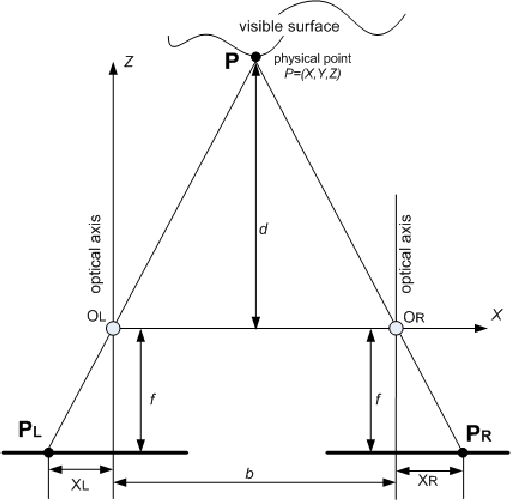
\includegraphics[height=0.5\textheight]{imgs/stereo.png}
		\end{center}
	\end{itemize}
	\end{frame}
	
	\begin{frame}
	\frametitle{Previous Works}
	\begin{itemize}
	
	\item \textit{Supervised Monocular Depth Estimation} : Early learning based approaches tend to segment the features of image and use some post processing steps. Deep learning based models have been successfully applied to single image depth estimation.However, training these models requires ground truth depth maps that are difficult to acquire.
	
		\begin{center}
			\begin{figure}
				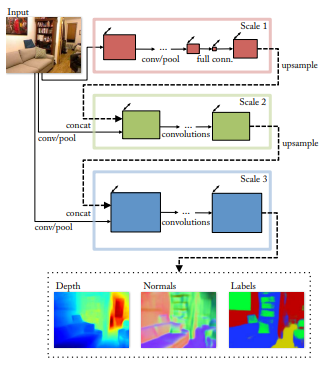
\includegraphics[height=0.4\textheight]{imgs/dl.png}
				\caption{\textcite{eigen2015predicting}}
			\end{figure}
			
		\end{center}
	
	\end{itemize}
	\end{frame}
	
	\begin{frame}
	\frametitle{Previous Works}
	\begin{itemize}
	
	\item \textit{Multi-view reconstruction} : Multi-view stereo algorithms estimate
	scene depth using multiple images captured from arbitrary view points. multi-view stereo techniques assume a static scene.
	For dynamic objects, these methods either produce erroneous estimates or drop pixels with low confidence. In contrast, our method
	produces dense depth even in the presence of moderate dynamic scene motion.
	\end{itemize}
	\end{frame}
	
	\begin{frame}
	\frametitle{Previous Works}
	\begin{itemize}
	
	\item \textit{Depth from video} : Recovering dense depth from monocular video is a challenging problem. To handle moving objects, existing techniques rely on motion segmentation and explicit motion modeling for the moving objects in the scene. 
	%(\textcite{casser2019depth})
	Several methods estimate depth by integrating motion estimation and multi-view reconstruction using two frames.The state-of-the-art video-to-depth methods predict a distribution over depth based on the cost volume constructed by warping nearby frames to a reference viewpoint. Such model designs thus do not account for dynamically moving objects.
	\end{itemize}
	
	\end{frame}
	
	
	
\end{document}